\documentclass[conference, utf8]{IEEEtran}
\IEEEoverridecommandlockouts
% The preceding line is only needed to identify funding in the first footnote. If that is unneeded, please comment it out.
\usepackage{cite}
\usepackage{amsmath,amssymb,amsfonts}
\usepackage{algorithmic}
\usepackage{graphicx}
\usepackage{textcomp}
\usepackage{xcolor}
\usepackage[hidelinks]{hyperref}
\usepackage{multirow}
\usepackage{float}
\usepackage[caption=false]{subfig}
\usepackage[font=small,labelfont=bf]{caption}
\usepackage[utf8]{inputenx}
\usepackage[croatian]{babel}
\def\BibTeX{{\rm B\kern-.05em{\sc i\kern-.025em b}\kern-.08em
		T\kern-.1667em\lower.7ex\hbox{E}\kern-.125emX}}
\begin{document}
	
	\title{Prepoznavanje raka pluća i debelog crijeva na slikama koristeći CNN}
	
	\author{\IEEEauthorblockN{1\textsuperscript{st} Dominik Jambrović}
		\IEEEauthorblockA{\textit{FER}}
		\and
		\IEEEauthorblockN{2\textsuperscript{nd} Filip Pankretić}
		\IEEEauthorblockA{\textit{FER}}
		\and
		\IEEEauthorblockN{3\textsuperscript{rd} Velimir Kovačić}
		\IEEEauthorblockA{\textit{FER}}
		\and
		\IEEEauthorblockN{4\textsuperscript{th} Filip Perković}
		\IEEEauthorblockA{\textit{FER}}
		\and
		\IEEEauthorblockN{5\textsuperscript{th} Luka Glavinić}
		\IEEEauthorblockA{\textit{FER}}
		\and
		\IEEEauthorblockN{6\textsuperscript{th} Neven Krznar}
		\IEEEauthorblockA{\textit{FER}}}
	
	\maketitle
	
	\section{Opis problema i motivacija}
	Rak je jedna od najsmrtonosnijih bolesti na svijetu. Svake godine izvještaji pokazuju preko 19 milijuna novih slučajeva i oko 10 milijuna smrtnih slučajeva \cite{world2019international}. Rak se može dobiti zbog mnogo razloga: UV zračenja, pušenja cigareta, udisanja kancerogenih plinova, nasljednih bolesti i tako dalje.
	\\
	Općenito stanice ljudskog tijela svaki dan umiru i zamjenjuju se novima procesom staničnog dijeljenja. Zbog trilijuna stanica koje čini naše tijelo, u ovim procesima može doći do greške pogrešnim repliciranjem molekule DNK.
	\\
	Upravo takve stanice se nazivaju tumorskim stanicama. Tumori mogu biti zloćudni ili dobroćudni. Zloćudni tumori dovode do raka koji može zahvatiti skoro pa svaki organ ljudskog tijela.
	\\
	Od raka obolijevaju i muškarci i žene, a najčešći oblici raka su: rak crijeva, rak pluća, rak jetre, rak dojke, rak rektuma, rak mozga, rak prostate, rak želuca i rak kože.
	\\
	Od raka pluća i raka crijeva otprilike jednakom mjerom obolijevaju i muškarci i žene, zbog čega će njihovo otkrivanje biti fokus ovoga rada.
	\\
	Za rak još uvijek nema lijeka, nego postoje samo tretmani koji mogu biti učinkoviti ako je rak otkriven što ranije.
	Zbog ovoga znanstvenici i doktori medicine diljem svijeta su počeli tražiti rješenje protiv ove bolesti u područjima dubokog učenja i računarske znanosti.
	\\
	Motivacija ovog rada je pokazati kako se pomoću umjetnih neuronskih mreža može obavljati bolje predviđanje prirode stanica tkiva slikanim medicinskim instrumentima i time pomoći stručnjacima dijagnosticirati pacijente.
	\\
	U ovome radu će se prvo opisati postojeća rješenja problema. Dalje, opisati korišteni skup podataka, a nakon toga korištene neuronske mreže i prikazati njihovi rezultati. Na kraju će se prodiskutirati i usporediti rezultati tuđih pristupa i našeg pristupa i dati zaključak.
	
	\section{Pregled postojećih rješenja}
	Prema \cite{mehmood2022malignancy} bilo je mnogo prijašnjih istraživanja na ovu temu i predloženih rješenja s obećavajućim rezultatima. U ovom poglavlju će se pričati o radovima s domenom o raku pluća i raku crijeva, jer je to tema našeg rada. Rješenja variraju po tipovima slika korištenih za treniranje modela, metodama za procesiranje slika, karakteristikama izvučenih iz svake slike i arhitekturama modela. U radu \cite{Sirinukunwattana} je predložena prostorno ograničena neuronska mreža za detektiranje jezgre u histopatološkim slikama stanica raka crijeva i postigla najveću točnost od 97.1\%. U radu \cite{Multimodal_sparse} je razvijena metoda za klasificiranje stanica raka iz jezgri stanica dobivenim biopsijom iglom i segmentiranim na 4372 regije. Postigli su konačnu točnost od 88.1\%. Također je razvijeno rješenje za višerazrednu klasifikaciju više tipova raka uz korištenje tri vrste stroja potpornih vektora(SVM) \cite{xu2013multi}. Dalje, u radu iz 2014.\cite{kuruvilla2014lung} predložena je CAD metoda za klasifikaciju raka pluća temeljena na dvije umjetne neuronske mreže, jedna s unaprijednom propagacijom, a druga s jednom unaprijednom i unatražnom propagacijom. Postignuta ukupna točnost je iznosila 93.3\%. Također u \cite{deppen2014accuracy} je razvijena metoda za analizu invazivnih plućnih čvorova pomoću slika dobivenih PET skeniranjem i dobivali visoku točnost njihovog otkrivanja. U 2016. opisana je prostorno ograničena CNN metoda za detekciju i klasifikaciju jezgara tumorskih stanica raka crijeva. Metoda funkcionira pomoću histopatoloških slika i bez potrebe segmentacije \cite{sirinukunwattana2016locality}. Metoda razvijena bez potrebe labeliranja slika za ocjenjivanje raka crijeva \cite{kuepper2016label}. U radu su korištene slike infracrvene histopatologije. Klasifikacija se radila pomoću nadziranog učenja temeljenog na stablu odluke. Ukupna dobivena točnost je iznosila 99\%. U 2017. je razvijena metoda za klasifikaciju zloćudnih čvorova pluća, za koju nije bila potrebna niti segmentacija niti izvlačenje značajki \cite{shen2017multi}. U cijelosti su se pouzdali u svoj model strojnog učenja i postigli točnost od 87.14\%. Dalje, prema \cite{sun2017automatic} je korištena i istrenirana konvolucijska neuronska mreža za otkrivanje prisustva raka pluća na 134,668 CT skenova. Postignuta je točnost od 89.9\%. Prema radu \cite{yuan2017automatic} je opisana metoda dubokog učenja za otkrivanje polipa iz videa kolonoskopije. Za klasifikaciju su koristili umjetnu neuronsku mrežu AlexNet što je rezultiralo s 91.47\% točnosti klasifikacije. Godine 2018. je predložena metoda za predviđanje raka pluća \cite{selvanambi2020lung} koristeći optimizaciju roja svitaca  (GSO) sa slikama iz različitih izvora i s rekurentnom neuronskom mrežom (RNN) kao algoritamom učenja. Dobili su maksimalnu točnost iznosa 98\%. \cite{de2018classification} je predložena metoda identifikacije raka pluća pomoću konvolucijske neuronske mreže i testirana na preko 50,500 slika CT skenova. Postignuta je točnost od 92.63\%. Prema radu \cite{da2020lung} predložena je metoda za identificiranje zloćudnih čvorova u plućima koristeći ResNet50 i postignuta je točnost od 93.19\%. U \cite{masood2018computer} je opisana razvijena CAD metoda za otkrivanje raka pluća i klasifikaciju stadija raka. Korištena je konvolucijska neuronska mreža(CNN) i DFCNet u ispitivanju na 6 drugačijih skupova podataka. Postignuta je točnost od 89.52\%. Nadalje, \cite{babu2018colon} je opisana RF-temeljen klasifikacijski model za predviđanje prisustva raka crijeva analizirajući histopatološke slike raka. Izvlačenje značajki su obavljali dekompozicijom valnih duljina slika. Postigli su maksimalnu točnost klasifikacije od 85.4\%. Rad \cite{mo2018efficient} opisuje metodu temeljenu na brzom R-CNN za pronalazak raka crijeva. Koristili su aproksimativnu zglobnu optimizaciju koja optimira klasifikacijske i regresijske gubitke istovremeno. Postigli su točnost od 98.5\%. Dalje, rad \cite{urban2018deep} je razvio metodu za klasifikaciju polipa iz slika kolonoskopije sa točnošću od 96\%. Koristili su konvolucijsku neuronsku mrežu treniranu na ručno labeliranim slikama od 2000 pacijenata. Godine 2019. je u radu \cite{shakeel2020automatic} je predstavljena metoda za automatsko otkrivanje raka pluća temeljena na slikama CT skenova. Najzanimljiviji dio ovog rada je da su autori koristili diskretnu "AdaBoost" optimiranu ansabl učilačku generaliziranu neuronsku mrežu ili DAELGNN i postigli impresivnu točnost od 99\%. Cilj rada \cite{toraman2019classification} je bio klasificirati izglednost raka crijeva pomoću infracrvenih Fourierovih tranformnih spektroskopskih signala. Autori su dobili nekoliko statističkih značajki iz tih signala i koristili stroj potpornih vektora(SVM) i umjetne neuronske mreže(ANN) da bi ih klasificirali i dobili točnost od 95.71\%. Godine 2020. Suresh i Mohan \cite{suresh2020roi} su opisali metodu za klasifikaciju raka pluća i dijagnozu vrste raka pomoću regije interesa(ROI) vrste učenja konvolucijske neuronske mreže. Dobili su točnost klasifikacije od 93.9\%. Nadalje, u radu \cite{masud2020light} je testiran model za otkrivanje plućnih čvorova temeljena na slikama CT skenova s plitkom konvolucijskom mrežom. Testirana je na LIDC skupu podataka, i dobivena klasifikacijska točnost od 97.9\%. \cite{shakeel2022automatic} je predložio još jednu metodu za otkrivanje raka pluća pomoću slika CT skenova. Micanjem šuma sa slika, uprijeli su unaprijeđenu konvolucijsku mrežu(IDNN) za segmentaciju slike i mnogo metoda ansambla(EM) za klasifikaciju slika i dobili točnost od 96.2\%.
	
	\section{Korišteni skup podataka}
	Za potrebe ovog rada, korišten je skup podataka \textit{LC25000}, objavljen 2020. \cite{borkowski2019lung} Sastoji se od 25000 slika tkiva pluća i debelog crijeva koje se dijele u 5 razreda:
	\begin{itemize}
		\item Adenokarcinom plućnog tkiva
		\item Karcinom pločastih (skvamoznih) stanica plućnog tkiva
		\item Dobroćudno (benigno) plućno tkivo
		\item Adenokarcinom tkiva debelog crijeva
		\item Dobroćudno (benigno) tkivo debelog crijeva
	\end{itemize}
	
	Skup se od 1250 jedinstvenih slika čiji je broj povećan rotacijama i zrcaljenjem na 25000. Svaki razred ima 5000 pripadnih slika. Sve su slike veličine 768 x 768 piksela. 
	
	\begin{figure}[H]
		\centering
		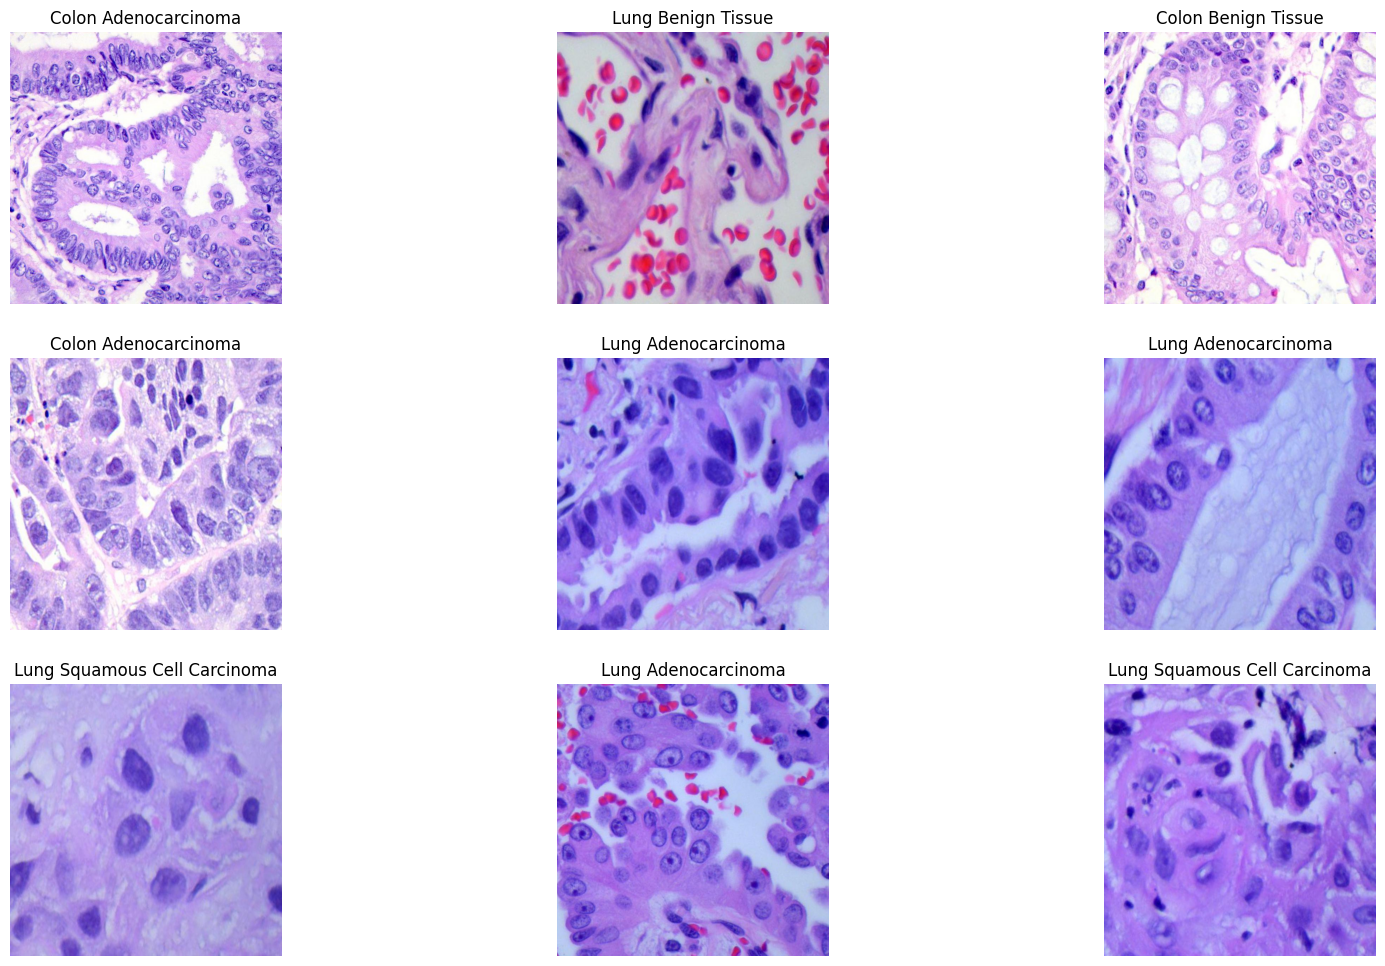
\includegraphics[width=\columnwidth]{ostalo/slike_tkiva.png}
		\caption{Prikaz 9 slučajno odabranih slika tkiva iz skupa podataka}
		\label{fig:tissue_images}
	\end{figure}
	
	\section{Konvolucijske neuronske mreže}
	Konvolucijska neuronska mreža inačica je višeslojnog perceptrona koja se temelji na filtriranju slike (konvoluciji). Mreža je nadahnuta povezanošću neurona u vidnoj kori ljudskog mozga.  Takva mreža je deterministička i pogodna za analizu slika. 
	
	Sastoji se od niza konvolucijskih slojeva isprekidanih slojevima sažimanja. Na kraju mreže može biti postavljen klasični višeslojni perceptron kojim se uspostavlja veza između mapi značajki i traženih izlaza. 
	
	\begin{figure}[H]
		\centering
		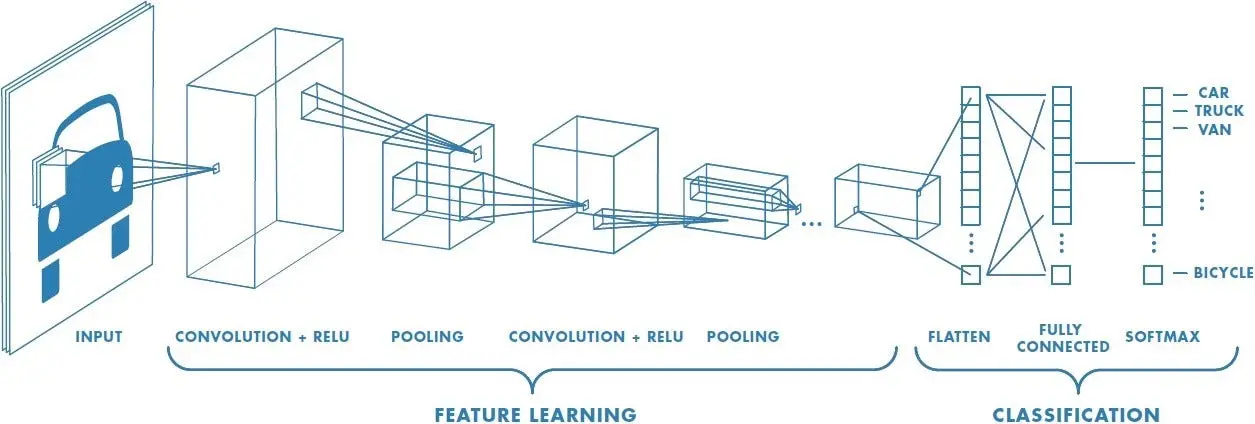
\includegraphics[width=\columnwidth]{ostalo/cnn.png}
		\caption{Primjer konvolucijske neuronske mreže za klasifikaciju vozila\cite{Saha_2023}}
		\label{fig:cnn}
	\end{figure}
	
	Konvolucijski sloj primjenjuje filtere (u obliku neurona) od kojih je svaki zadužen za pojedinu značajku. Rezultat primjene tih filtara naziva se mapa značajki. Svaki se filter primjenjuje na svim mapama značajki prethodnog sloja, a pritom su težine neurona iste ili slične. Takav sloj je neovisan o translaciji, ali ima ograničenu robusnost na rotaciju. 
	
	Sloj sažimanja služi za smanjenje veličine ulaza. Uz to umanjuje utjecaj pomaka značajki u prostoru.
	
	Konvolucijska neuronska mreža uči se postupkom propagacije unatrag (često uz korištenje minigrupa). Kod propagacije unatrag postoji problem iščezavanja gradijenta zbog velikog broja slojeva. Prilikom praktične izvedbe učenja često je problem nedostatak memorije GPU. Može se zaobići korištenjem slobodno dostupnih predtreniranih slojeva mreže.
	
	\section{Materijali i metode}
	Skup podataka \textit{LC25000} podijeljen je na 3 disjunktna podskupa: skup za učenje (70\% podataka), skup za validaciju (10\% podataka) i skup za testiranje ((20\% podataka)). Skup za validaciju služi za odabir optimalnog modela prilikom učenja, a skup za testiranje služi za mjerenje performansi modela na neviđenim podacima. Same slike nisu prilagođavane, nego dovođene na ulaz neuronske mreže onakve kakve jesu. Dodatno, prilikom učenja korištene su minigrupe od po 16 slika. Korištena su 2 modela: \textit{ResNet50} i \textit{MobileNetV2}. 
	
	Radi povećanja učinkovitosti, modeli su inicijalizirani mrežama predtreniranim na skupu podataka \textit{ImageNet}. To je skup s preko 14 milijuna slika i više od 20 tisuća razreda. 
	
	\subsection{ResNet50}
	Kao temelj prvog modela korištena je konvolucijska neuronska mreža s 50 slojeva \textit{ResNet50}. Ona ima 48 konvolucijskih slojeva, jedan sloj \textit{MaxPool} i jedan sloj \textit{Average pooling}. 
	
	Glavna inovacija u \textit{ResNet50} su rezidualne veze, koje omogućavaju mreži da nauči rezidualne funkcije za mapiranje ulaza na tražene izlaze. Omogućava veću dubinu mreža bez problema iščezavanja gradijenta. 
	
	Prednaučena je na skupu podataka \textit{ImageNet}. Dodano je još 4 skrivena te 1 izlazni sloj. Skriveni slojevi su redom: \textit{BatchNormalization}, \textit{Flatten}, potpuno povezani sloj \textit{Dense} s aktivacijskom funkcijom \textit{ReLu} i \textit{Dropout}. Izlazni sloj je potpuno povezani sloj \textit{Dense} s aktivacijskom funkcijom \textit{softmax}.
	
	\begin{figure}[H]
		\centering
		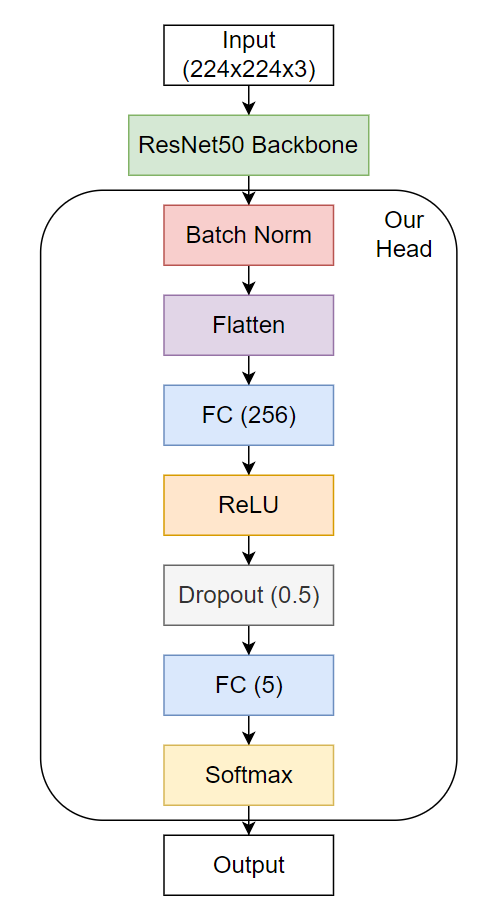
\includegraphics[width=0.5\columnwidth]{ostalo/resnet50model.png}
		\caption{Arhitektura korištenog modela ResNet50}
		\label{fig:resnet50model}
	\end{figure}
	
	Dakle model \textit{ResNet50} ima 55 slojeva i 49287557 parametara, od kojih je 25695749 njih učivo jer se predtrenirani slojevi nisu učili. Učenje modela provedeno je kroz 60 epoha.
	
	
	
	\subsection{MobileNetV2}
	Drugi model utemeljen je na čisto konvolucijskoj neuronskoj mreži s 53 konvolucijska sloja \textit{MobileNetV2}. Ona je osmišljena kako bi učinkovita radila na mobilnim uređajima zahvaljujući manjem broju parametara. Uvodi novu vrstu bloka \textit{Inverted Residuals} i konvolucijski sloj \textit{Linear Bottleneck}. U bloku \textit{Inverted Residuals}, značajke nižih dimenzija preslikavaju se u više dimenzije, zatim se primjenjuje konvolucijski sloj \textit{Depthwise}, nakon čega se dimenzije značajki ponovno snižavaju na početne. Sloj \textit{Linear Bottleneck} konvolucijski je sloj \textit{Bottleneck} s linearnom aktivacijskom funkcijom.
	
	Prednaučena je na skupu podataka \textit{ImageNet}. Dodano je još 2 skrivena te 1 izlazni sloj. Skriveni slojevi su  \textit{BatchNormalization} i \textit{Flatten}. Izlazni sloj je \textit{Dense} s aktivacijskom funkcijom \textit{softmax}.
	
	\begin{figure}[H]
		\centering
		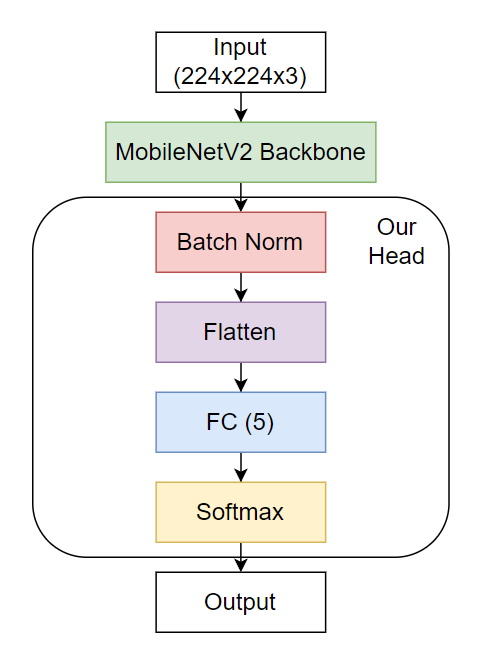
\includegraphics[width=0.5\columnwidth]{ostalo/mobilenetv2model.png}
		\caption{Arhitektura korištenog modela MobileNetV2}
		\label{fig:mobilenetv2model}
	\end{figure}
	
	Dakle model \textit{MobileNetV2} ima 56 slojeva i 2576709 parametara, od kojih je 2540037 njih učivo. Za razliku od modela \textit{ResNet50}, uče se i prednaučeni slojevi. Učenje modela provedeno je kroz 60 epoha.
	
	\section{Rezultati i usporedba s prijašnjim radovima}
	\subsection{Prijašnji radovi}
	Radovi s kojima će se rezultati uspoređivati su \cite{RAD1} i \cite{RAD2}. 
	
	U radu \cite{RAD1} koristi se konvolucijska neuronska mreža \textit{AlexNet} s preko 60 milijuna parametara (za usporedbu \textit{ResNet50} ima nešto manje od 50 milijuna). Sastoji se od 5 konvolucijskih slojeva i 3 potpuna povezana sloja. Skup podataka podijeljen je na skup za učenje (80\%) i skup za testiranje (20\%). Učenje je provedeno kroz 60 epoha. Na slikama iz razreda s lošijim rezultatima,  primijenjena je metoda \textit{Histogram equalization} radi poboljšanja kontrasta. Taj postupak naziva se CSIP (\textit{Class Selective Image Processing}).
	
	U \cite{RAD2} glavni je fokus na pretprocesiranju skupa podataka. Povećava se oštrina slika metodom USM (\textit{Unsharp masking}) i radi se izlučivanje 2D Fourierovih značajki i 2D \textit{Wavelet} značajki koje se na kraju kombiniraju. Koristi se vlastita konvolucijska neuronska mreža s 3 konvolucijska sloja, 2 sloja \textit{MaxPool}, slojem \textit{BatchNormalization} i slojem \textit{Dropout}. Učenje je provedeno kroz 500 epoha. Skup podataka podijeljen je na skup za učenje (70\%) i skup za testiranje (30\%)
	
	
	
	
	\subsection{Točnost i gubitak}
	Za oba modela prikazani su grafovi točnosti i gubitka na skupu za učenje i skupu za validaciju tijekom procesa učenja (slike \ref{fig:RN50_acc_loss} i \ref{fig:MN_acc_loss}). 
	\begin{figure}[H]
		\centering
		\includegraphics[width=\columnwidth]{ResNet50/accuracy_loss.png}
		\caption{Točnost (lijevo) i gubitak (desno) modela ResNet50 nad podacima za treniranje i validaciju po epohama}
		\label{fig:RN50_acc_loss}
	\end{figure}
	\begin{figure}[H]
		\centering
		\includegraphics[width=\columnwidth]{MobileNetV2/accuracy_loss.png}
		\caption{Točnost (lijevo) i gubitak (desno) modela MobileNetV2 nad podacima za treniranje i validaciju po epohama}
		\label{fig:MN_acc_loss}
	\end{figure}
	
	Tablicom \ref{table:1} usporedno su prikazane točnosti predviđanja naših modela i modela iz prijašnjih radova nakon učenja. 	
	Primjetno je da model \textit{ResNet50} ima veću točnost (99.32\%) na skupu za testiranje od modela \textit{MobileNetV2} (98.65\%), ali i da oba imaju veću točnost od modela iz prijašnjih radova \cite{RAD1} i \cite{RAD2}.
	
	\begin{table}[H]
		\centering
		\caption{Usporedni prikaz točnosti modela}
		\label{table:1}
		\begin{tabular}{ |c|c|c| } 
			\hline
			& \multicolumn{2}{c|}{Točnost} \\
			\hline
			Model & Skup za učenje  & Skup za testiranje \\
			\hline \hline
			\textbf{ResNet50} & \textbf{99.45\%}  & \textbf{99.32\%}  \\
			\hline
			MobileNetV2 & 99.78\%  & 98.65\%  \\
			\hline
			AlexNet\cite{RAD1} & 99.85\%  & 98.40\%  \\
			\hline
			CNN\cite{RAD2} & 98.87\% & 96.33\%  \\
			\hline
		\end{tabular}
	\end{table}
	
	\subsection{Matrica zabune}
	Matrice zabune, računate na skupu za testiranje, prikazane su za oba naša modela (slike \ref{conf:1} i \ref{conf:2}). Uz to prikazane su i matrice zabune modela iz radova \cite{RAD1} i \cite{RAD2} (slike \ref{conf:3} i \ref{conf:4}).
	
	Radi lakšeg snalaženja na matrici zabune, u tablici \ref{table:3} predstavljene su brojčane oznake pojedinih razreda.
	
	\begin{table}[H]
		\centering
		\caption{Oznake razreda na grafu}
		\label{table:3}
		\begin{tabular}{ |c|c| } 
			\hline
			Oznaka & Razred \\
			\hline \hline
			0 & Adenokarcinom tkiva debelog crijeva \\
			\hline
			1 & Dobroćudno (benigno) tkivo debelog crijeva \\
			\hline
			2 & Adenokarcinom plućnog tkiva \\
			\hline
			3 & Dobroćudno (benigno) plućno tkivo \\
			\hline
			4 & Karcinom pločastih (skvamoznih) stanica plućnog tkiva \\
			\hline
		\end{tabular}
	\end{table}
	
	
	\begin{figure}[H]
		
		\begin{center}
			\begin{minipage}{0.49\columnwidth}
				\includegraphics[width=\columnwidth]{ResNet50/confusion_matrix.png}
				\captionof{figure}{ResNet50}
				\label{conf:1}
			\end{minipage}
			\begin{minipage}{0.49\columnwidth}
				\includegraphics[width=\columnwidth]{MobileNetV2/confusion_matrix.png}
				\captionof{figure}{MobileNetV2}
				\label{conf:2}
			\end{minipage}
			\begin{minipage}{0.49\columnwidth}
				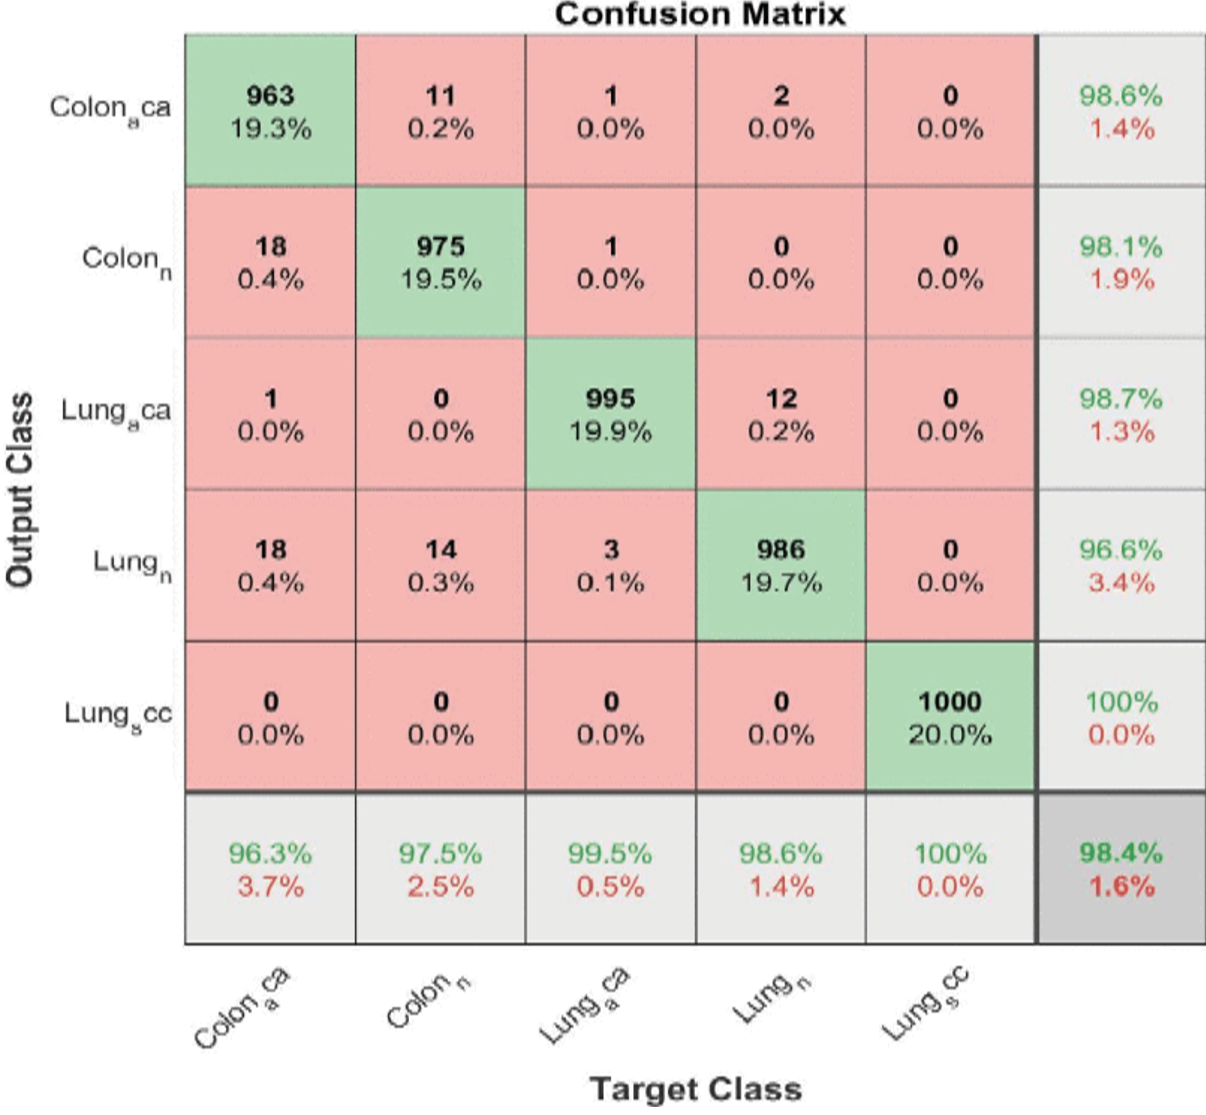
\includegraphics[width=\columnwidth]{ostalo/rad1_conf.png}
				\captionof{figure}{AlexNet\cite{RAD1}}
				\label{conf:3}
			\end{minipage}
			\begin{minipage}{0.49\columnwidth}
				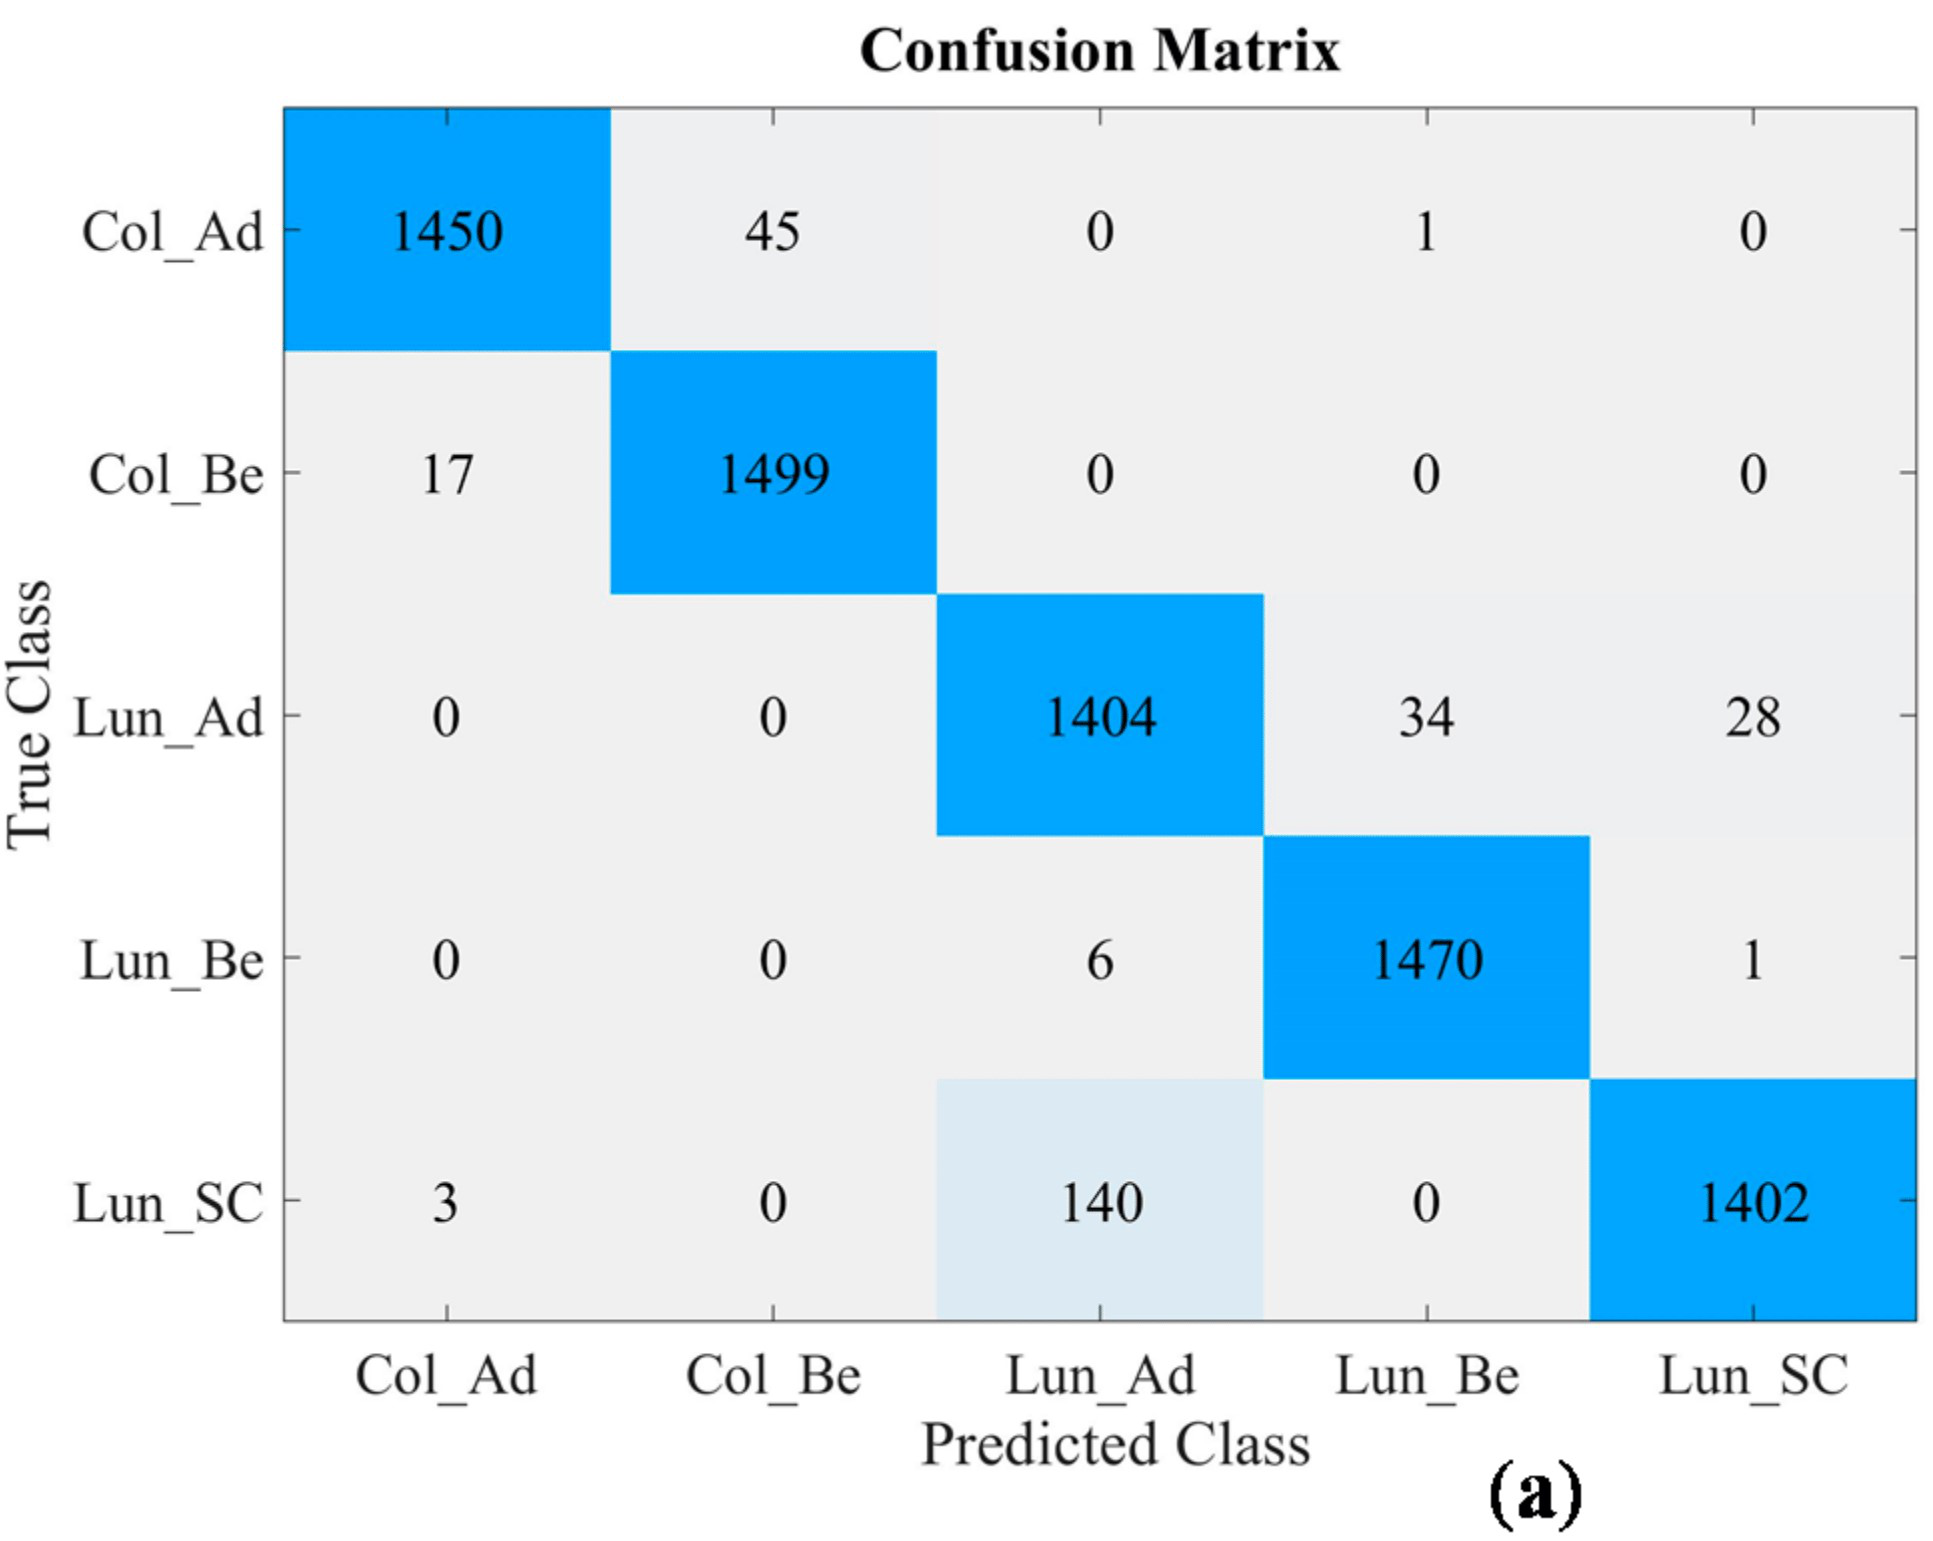
\includegraphics[width=\columnwidth]{ostalo/rad2_conf.png}
				\captionof{figure}{CNN\cite{RAD2}}
				\label{conf:4}
			\end{minipage}
			
			
		\end{center}
		
		\caption{Matrice zabune 4 razmatrana modela}
		
	\end{figure}
	
	
	
	
	
	
	Model \textit{ResNet50} ima općenito najmanje pogrešnih klasifikacija, 0.68\%. \textit{MobileNetV2} ima 1.16\%, \textit{AlexNet}\cite{RAD1} ima 1.62\%  i \textit{CNN}\cite{RAD2} ima 3.67\% pogrešnih klasifikacija. 
	
	\textit{ResNet50}, \textit{MobileNetV2} i \textit{CNN}\cite{RAD2} imaju problema s razlikovanjem adenokarcinoma i karcinoma pločastih stanica plućnog tkiva. Uspješno raspoznaje radi li se o karcinomu ili ne, ali teže određuje vrstu karcinoma na plućnom tkivu. To implicira bliskost tih grupa slika u ulaznom prostoru i odgovara prirodi problema.
	
	\textit{AlexNet}\cite{RAD1} taj problem nema, ali ima više manjih pogrešaka između raznih razreda. 
	
	
	
	\section{Mjere dobrote}
	Konačno, za svaki razred u oba naša modela dan je stupčasti dijagram sljedećih mjera dobrote: točnost (\ref{eq:1}), preciznost (\ref{eq:2}), F1 (\ref{eq:4}), odziv (\ref{eq:3}) i specifičnost (\ref{eq:5}) (slike \ref{fig:RN50_fit_met} i \ref{fig:MN_fit_met}). Isti podaci prikazani su tablično (tablice \ref{table:4} i \ref{table:5}). Tablica \ref{table:6} usporedno prikazuje prosječne mjere dobrote nad svim klasama za naše modele i modele iz prijašnjih radova.
	
	\begin{equation}
		Accuracy = \frac{TP + TN}{TP + TN + FP + FN} \label{eq:1}
	\end{equation}
	\begin{equation}
		Precision = \frac{TP}{TP + FP} \label{eq:2}
	\end{equation}
	\begin{equation}
		Recall = \frac{TP}{TP + FN} \label{eq:3}
	\end{equation}
	\begin{equation}
		F1 = \frac{TP}{TP + 0.5(FN + FP)}\label{eq:4}
	\end{equation}
	\begin{equation}
		Specificity = \frac{TN}{TN + FP} \label{eq:5}
	\end{equation}
	
	
	\begin{figure}[H]
		\centering
		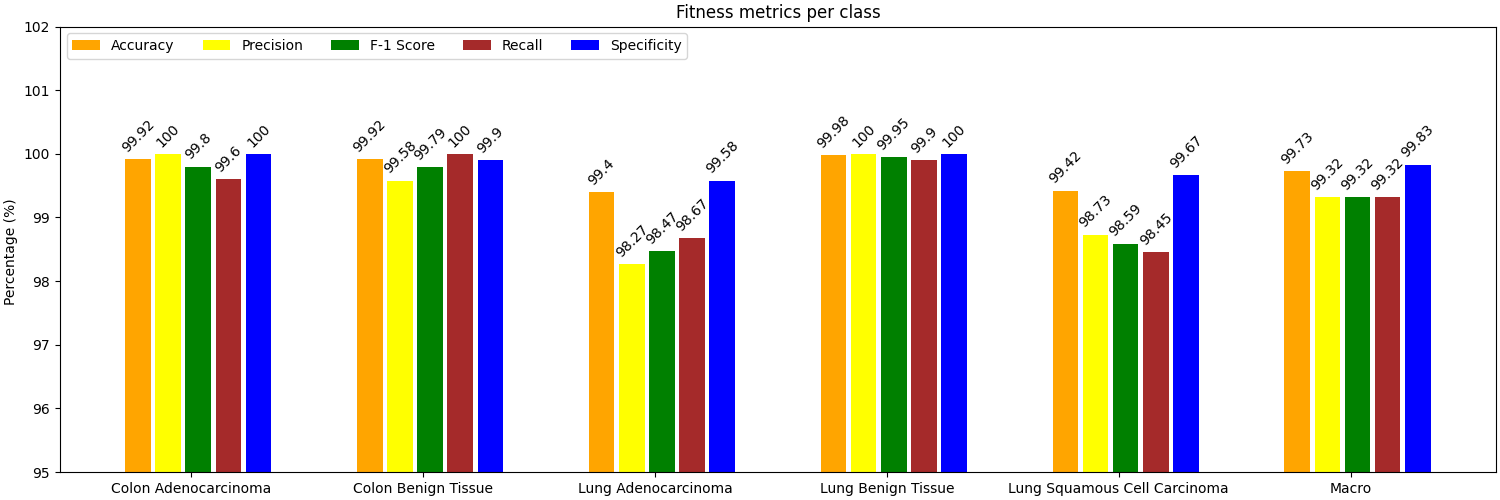
\includegraphics[width=\columnwidth]{ResNet50/fitness_metrics.png}
		\caption{Mjere dobrote modela ResNet50}
		\label{fig:RN50_fit_met}
	\end{figure}
	
	
	
	\begin{figure}[H]
		\centering
		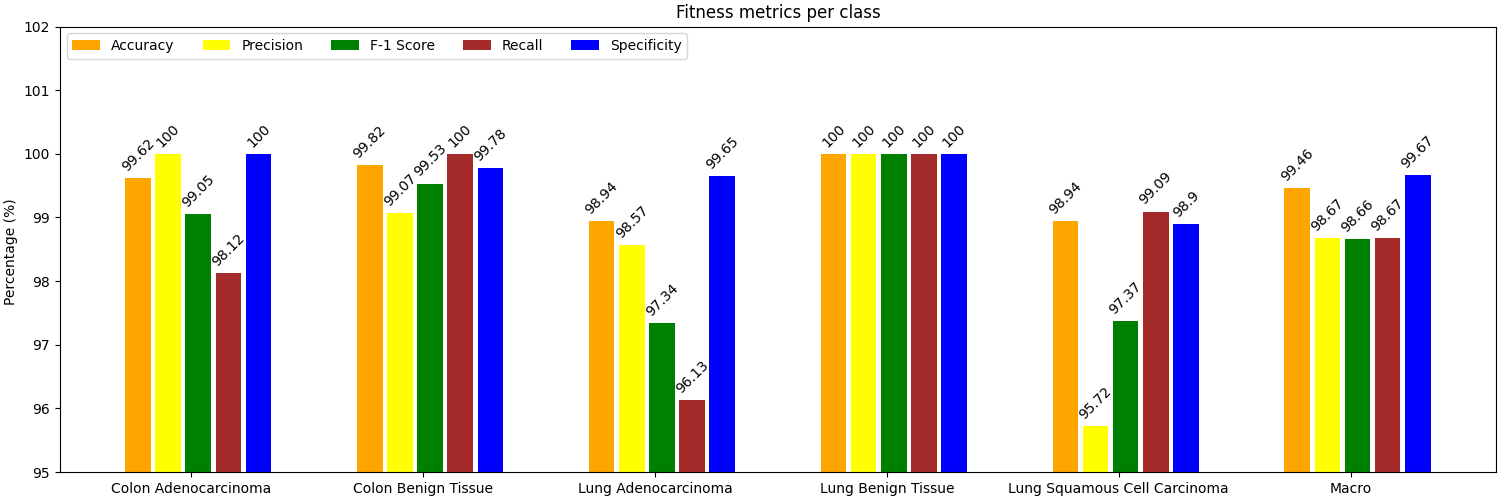
\includegraphics[width=\columnwidth]{MobileNetV2/fitness_metrics.png}
		\caption{Mjere dobrote modela MobileNetV2}
		\label{fig:MN_fit_met}
	\end{figure}
	
	%	\begin{figure}[ht]
		%		\centering
		%		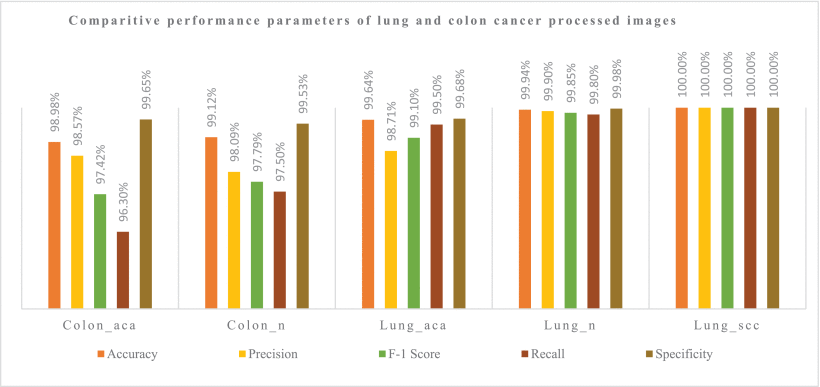
\includegraphics[width=\columnwidth]{ostalo/rad1_stupci.png}
		%		\caption{Mjere dobrote modela AlexNet\cite{RAD1}}
		%		\label{fig:AlexNet_fit_met}
		%	\end{figure}
	
	
	
	\begin{table}[H]
		\centering
		\caption{Mjere dobrote razreda za model ResNet50}
		\label{table:4}
		\begin{tabular}{ |c|c|c|c|c|c| } 
			\hline
			Razred & Točnost & Preciznost & F1 & Odziv & Specifičnost \\
			\hline\hline
			0 & 99.92\% & 100\% & 99.8\% & 99.6\% & 100\% \\
			\hline
			1 & 99.92\% & 99.58\% & 99.79\% & 100\% & 99.9\% \\
			\hline
			2 & 99.4\% & 98.27\% & 98.47\% & 98.67\% & 99.58\% \\
			\hline
			3 & 99.98\% & 100\% & 99.95\% & 99.9\% & 100\% \\
			\hline
			4 & 99.98\% & 100\% & 99.95\% & 99.9\% & 100\% \\
			\hline
		\end{tabular}
	\end{table}
	\begin{table}[H]
		\centering
		\caption{Mjere dobrote razreda za model MobileNetV2}
		\label{table:5}
		\begin{tabular}{ |c|c|c|c|c|c| } 
			\hline
			Razred & Točnost & Preciznost & F1 & Odziv & Specifičnost \\
			\hline\hline
			0 & 99.62\% & 100\% & 99.05\% & 98.12\% & 100\% \\
			\hline
			1 & 99.82\% & 99.07\% & 99.53\% & 100\% & 99.78\% \\
			\hline
			2 & 98.94\% & 98.57\% & 97.34\% & 96.13\% & 99.65\% \\
			\hline
			3 & 100\% & 100\% & 100\% & 100\% & 100\% \\
			\hline
			4 & 98.94\% & 95.72\% & 97.37\% & 99.09\% & 98.9\% \\
			\hline
		\end{tabular}
	\end{table}
	
	Kao i prilikom analize matrica zabune, može se vidjeti da su mjere oba modela lošije kada se razmatraju razredi karcinoma plućnog tkiva. Oba modela teže raspoznaju karcinom pločastih stanica i adenokarcinom plućnog tkiva. \textit{MobileNetV2} ima lošije mjere od \textit{ResNet50} na svim razredima osim na dobroćudnom plućnom tkivu, koje je klasificirao potpuno točno. 
	
	
	\begin{table}[H]
		\centering
		\caption{Prosječne mjere dobrote za sve modele}
		\label{table:6}
		\begin{tabular}{ |c|c|c|c|c| } 
			\hline
			Model & Točnost & Preciznost & F1 &;   Specifičnost \\
			\hline\hline
			\textbf{ResNet50} & \textbf{99.73\%} & \textbf{99.32\% }& \textbf{99.32\%} &  \textbf{99.83\%} \\
			\hline
			MobileNetV2 & 99.46\% & 98.67\% & 98.66\% &;  99.67\% \\
			\hline
			AlexNet\cite{RAD1} & 95.90\% &	92.36\%	&86.94\% &	97.46\%
			\\
			\hline
			CNN\cite{RAD2} & 96.33\% & 96.39\% & 96.38\% & 96.37\% \\
			\hline
		\end{tabular}
	\end{table}
	
	Usporednom analizom mjera naših modela i modela iz prijašnjih radova, vidi se da naši modeli imaju bolji rezultat po svim korištenim mjerilima.
	
	
	
	
	\section{Zaključak}
	U ovom radu su opisane dvije metode za klasifikaciju dvije varijante raka pluća i raka crijeva pomoću dvije mreže, i klasifikacija bezopasnih stanica tkiva. Opisani su podaci nad kojima su metode testirane i opisani su prijašnji radovi koji su predložili rješenja na temu. Nakon provedenih eksperimenata su opisani vrlo zadovoljavajući rezultati i dane su usporedbe s prijašnjim radovima. Naša metoda je u usporedbi na rad koji smo uzeli za glavni uzor dala i bolje rezultate. Također smo predstavili metodu koja ne samo da ne iziskuje pretprocesiranje slika, već i sadrži izrazito manji skup parametara(MobileNetV2), što daje motivaciju za daljnja istraživanja s njime i laku mobilizaciju i primjenu u stvarnoj medicinskoj industriji. Ovo je područje koje se ubrzanim tempom širi, i sadrži još mnogo prostora za daljnji rast i novog proučavanja. Radovi na ovu temu su od izrazite važnosti jer mogu spasiti milijune ljudskih života od ove strašne bolesti.
	
	\bibliography{literatura}
	\bibliographystyle{ieeetr}
\end{document}